\documentclass[aspectratio=169]{beamer}
\usepackage{graphicx}
\usepackage{color}
\usepackage{multimedia} 
\usepackage{helvet}
\renewcommand\familydefault{\sfdefault}
\usepackage{sansmath}
\usepackage[normalem]{ulem}
% Settings
\definecolor{darkgray}{RGB}{30, 30, 30}
\setbeamercolor{normal text}{fg=white,bg=black}
\setbeamercolor{alerted text}{fg=white}
\setbeamercolor{structure}{fg=white}
\setbeamercolor{title}{fg=white}
\setbeamercolor{frametitle}{fg=white}
\setbeamercolor{item}{fg=white}
\setbeamercolor{subitem}{fg=white}
\setbeamercolor{page number in head/foot}{fg=white}
\setbeamerfont{title}{size=\fontsize{48}{48}\selectfont}
\setbeamerfont{frametitle}{size=\fontsize{20}{10}\selectfont,series=\bfseries}
\setbeamerfont{itemize/enumerate body}{size=\fontsize{16}{16}\selectfont}
\setbeamerfont{itemize/enumerate subbody}{size=\fontsize{14}{14}\selectfont}
\setbeamerfont{normal text}{size=\fontsize{24}{24}\selectfont}
\setbeamerfont{column}{size=\fontsize{20}{20}\selectfont}
\setbeamertemplate{navigation symbols}{}
\setbeamertemplate{footline}{%
	\hfill\insertframenumber\hspace{10pt}\vspace{8pt}
}
\setbeamertemplate{frametitle}{%
	\vspace*{-0.4em}% Remove top whitespace
	\nointerlineskip
	\begin{beamercolorbox}[wd=\paperwidth,ht=3ex,dp=1.5ex,leftskip=1em, left]{frametitle}
		\usebeamerfont{frametitle}\hspace{0.2em}\insertframetitle
	\end{beamercolorbox}%
}
\newcommand{\ct}[1]{\uline{#1}\\}
\newcommand{\cc}[1]{\textbf{#1} \\}
%\newcommand{\ccc}[1]{\quad - #1\\}
\newcommand{\ccc}[1]{%
  \par\hangindent=2em\hangafter=1\hspace{0.5em} - #1\par\smallskip
}
% Set line spread and parskip
\linespread{1.05}
\begin{document}

\begin{frame}{Macau story}
	\begin{center}
		\includegraphics[width=\textwidth,height=0.9\textheight,keepaspectratio]{macau.jpg}
	\end{center}
\end{frame}

\begin{frame}{Macau story: Simplified}
	\vspace{-2em}
	\begin{columns}[T]
		\begin{column}{0.4\textwidth}
			\centering
			\includegraphics[width=\textwidth,height=0.9\textheight,keepaspectratio]{cointoss.png}
		\end{column}
		\hfill
		\begin{column}{0.6\textwidth}\large
			\cc{Suppose}
			\ccc{We toss the coin 10 times and get 8 heads}
			\cc{Has the Casino rigged the coin?}
		\end{column}
	\end{columns}
\end{frame}


\begin{frame}{Macau story}
	\vspace{-2em}
	\begin{columns}[T]
		\begin{column}{0.4\textwidth}
			\centering
			\includegraphics[width=\textwidth,height=0.9\textheight,keepaspectratio]{cointoss.png}
		\end{column}
		\hfill
		\begin{column}{0.6\textwidth}\large
			\cc{Suppose}
			\ccc{The probability that a coin returns head is 0.5}
			\ccc{We toss the coin 10 times and get 8 heads}
			\cc{What is the probability of getting 8 heads in 10 tosses?}
		\end{column}
	\end{columns}
\end{frame}

\begin{frame}{Macau story: Simplified}
	\vspace{-2em}
	\begin{columns}[T]
		\begin{column}{0.4\textwidth}
			\centering
			\includegraphics[width=\textwidth,height=0.9\textheight,keepaspectratio]{cointoss.png}
		\end{column}
		\hfill
		\begin{column}{0.6\textwidth}\large
			\cc{Suppose}
			\ccc{The probability that a coin returns head is 0.5}
			\ccc{We toss the coin 10 times and get 8 heads}
			\cc{What is the probability of getting 8 heads in 10 tosses?}
			\ccc{Answer:}
			$$P(T=8) = \binom{10}{8}\cdot 0.5^8 \cdot (1-0.5)^{10-8} = 45/1024$$
			$$\approx 0.044 \quad\quad(\text{around }4.4\%)$$
			\cc{More likely to be rigged?}
		\end{column}
	\end{columns}
\end{frame}

% Now do the same question but with probability p instead of 0.5
\begin{frame}{Introducing competing hypotheses}
	\vspace{-2em}
	\begin{columns}[T]
		\begin{column}{0.4\textwidth}
			\centering
			\includegraphics[width=\textwidth,height=0.9\textheight,keepaspectratio]{cointoss.png}
		\end{column}
		\hfill
		\begin{column}{0.7\textwidth}\large
			$$H_\text{fair}:\quad \text{The coin is fair}$$
			$$H_\text{rigged}:\quad \text{The coin is rigged}$$
			\cc{Probability of observing the data (8 heads in 10 tosses) under each hypothesis:}
			$$P(T|H_\text{fair},N) = \binom{N}{T} \cdot (0.5)^T \cdot (1-0.5)^{N-T}$$
			$$P(T|H_\text{rigged},q,N) = \binom{N}{T} \cdot q^T \cdot (1-q)^{N-T}$$
			coin bias $q$ is the probability of getting heads under the rigged hypothesis.\\
			\cc{Under which hypothesis is the data more likely?}
			\ccc{Assume total ignorance for $q$}
		\end{column}
	\end{columns}
\end{frame}

% Compute the Bayes factor:
\begin{frame}{Bayes factor}
	\vspace{-2em}
	\begin{columns}[T]
		\begin{column}{0.4\textwidth}
			\centering
			\includegraphics[width=\textwidth,height=0.9\textheight,keepaspectratio]{cointoss.png}
		\end{column}
		\hfill
		\begin{column}{0.7\textwidth}\large
			\cc{Bayes factor:}
			$$B^r_f = \frac{P(T|H_\text{rigged},N)}{P(T|H_\text{fair},N)}$$ 
			\cc{Evidence under rigged hypothesis:}
			$$P(T|H_\text{rigged},N) = \int_0^1 P(T|H_\text{rigged},q,N) \cdot P(q|H_\text{rigged}) dq$$
			\cc{Total ignorance for $q$: $P(q|H_\text{rigged}) = 1$}
			$$P(T|H_\text{rigged},N) = \frac{1}{N+1}$$
			$$B^r_f \approx 2$$
		\end{column}
	\end{columns}
\end{frame}

\begin{frame}{Is the coin rigged though?}
	\vspace{-2em}
	\begin{columns}[T]
		\begin{column}{0.4\textwidth}
			\centering
			\includegraphics[width=\textwidth,height=0.9\textheight,keepaspectratio]{cointoss.png}
		\end{column}
		\hfill
		\begin{column}{0.7\textwidth}\large
			\cc{The Bayes factor is two. What does this mean?}
			\ccc{The data is twice as likely under the rigged hypothesis than under the fair hypothesis.}
			\cc{Is this strong evidence for the rigged hypothesis?}
			\ccc{Not really.}
			\ccc{For example, repeating the experiment 10 times would likely yield at least one experiment with a Bayes factor of 2 or more, even if the coin is fair.}
		\end{column}
	\end{columns}
\end{frame}


\begin{frame}{Repeating the experiment 7 times}
	\vspace{-2em}
	\begin{columns}[T]
		\begin{column}{0.4\textwidth}
			\centering
			\includegraphics[width=\textwidth,height=0.9\textheight,keepaspectratio]{cointoss.png}
		\end{column}
		\hfill
		\begin{column}{0.7\textwidth}\large
			\cc{You repeat the experiment 7 times, each experiment gives 8 tails in 10 tosses.}
			\ccc{Is the coin rigged?}
		\end{column}
	\end{columns}
\end{frame}

\begin{frame}{Surely it's rigged now?}
	\vspace{-2em}
	\begin{columns}[T]
		\begin{column}{0.4\textwidth}
			\centering
			\includegraphics[width=\textwidth,height=0.9\textheight,keepaspectratio]{cointoss.png}
		\end{column}
		\hfill
		\begin{column}{0.7\textwidth}\large
			\cc{You have ten datasets $\vec d$}
			\ccc{Let us assume that the datasets are independent}
			$$P(\vec d|H_\text{rigged},N) = \prod_{i=1}^{10} P(d_i|H_\text{rigged},N)$$
			$$P(\vec d|H_\text{fair},N) = \prod_{i=1}^{10} P(d_i|H_\text{fair},N)$$
			$$B^r_f \approx (2.068\cdots)^7 \approx 162$$
			\ccc{Is the coin rigged now?}
		\end{column}
	\end{columns}
\end{frame}

\begin{frame}{Surely it's rigged now?}
	\vspace{-2em}
	\begin{columns}[T]
		\begin{column}{0.4\textwidth}
			\centering
			\includegraphics[width=\textwidth,height=0.9\textheight,keepaspectratio]{rigged_news.png}
		\end{column}
		\hfill
		\begin{column}{0.7\textwidth}\large
			\cc{You repeat the experiment 8 times, each experiment gives 8 tails in 10 tosses.}
			\ccc{Is the coin rigged?}
			\ccc{A rigged coin is around 162 times more likely to generate the data than a fair coin.}
			\cc{It's still probably not rigged. Why?}
			\ccc{See the news story on the left}
		\end{column}
	\end{columns}
\end{frame}

\begin{frame}{Posterior odds}
	\vspace{-2em}
	\begin{columns}[T]
		\begin{column}{0.4\textwidth}
			\centering
			\includegraphics[width=\textwidth,height=0.9\textheight,keepaspectratio]{rigged_news.png}
		\end{column}
		\hfill
		\begin{column}{0.7\textwidth}\large
			\vspace{-1em}
			\cc{Bayes factor is not the end of the story.}
			\ccc{We also need to consider the prior odds:}
			$$O^r_f = \frac{P(H_\text{rigged}|\vec d, {\color{blue}I})}{P(H_\text{fair}|\vec d,{\color{blue}I})}$$
			$$= \frac{P(\vec d|H_\text{rigged},{\color{blue}I})}{P(\vec d|H_\text{fair},{\color{blue}I})} \cdot \frac{P(H_\text{rigged}|{\color{blue}I})}{P(H_\text{fair}|{\color{blue}I})} = 162 \cdot \frac{P(H_\text{rigged}|{\color{blue}I})}{P(H_\text{fair}|{\color{blue}I})}$$
			\cc{Only $<$ 1 in 10,000 casinos are rigged}
			\ccc{Macau Casinos are heavily regulated.}
			\ccc{Prior odds of rigged vs fair: $1/10,000$}
			$$O^r_f = 162 \cdot \frac{1}{10,000} = 0.0162\approx1/200$$
			\cc{Conclusion: The coin is still probably not rigged.}
		\end{column}
	\end{columns}
\end{frame}


\begin{frame}{Home casino}
	\vspace{-2em}
	\begin{columns}[T]
		\begin{column}{0.4\textwidth}
			\centering
			\includegraphics[width=\textwidth,height=0.9\textheight,keepaspectratio]{homecasino.png}
		\end{column}
		\hfill
		\begin{column}{0.7\textwidth}\large
			\vspace{-2em}
			\cc{Home casino}
			\ccc{You hear from around 50\% of your friends who plays at the casino that the casino cheats.}
			\cc{You get 8 heads in 10 tosses, 8 times in a row.}
			\ccc{Is the coin rigged now?}
			$$O^r_f = \frac{P(H_\text{rigged}|\vec d, {\color{blue}I})}{P(H_\text{fair}|\vec d,{\color{blue}I})}$$
			$$= \frac{P(\vec d|H_\text{rigged},{\color{blue}I})}{P(\vec d|H_\text{fair},{\color{blue}I})} \cdot \frac{P(H_\text{rigged}|{\color{blue}I})}{P(H_\text{fair}|{\color{blue}I})} = 162 \cdot \frac{P(H_\text{rigged}|{\color{blue}I})}{P(H_\text{fair}|{\color{blue}I})}$$
			\cc{Prior odds of rigged vs fair: $1/1$}
			$$O^r_f = 162 \cdot \frac{1}{1} = 162$$
			\cc{Conclusion: The coin is probably rigged.}
		\end{column}
	\end{columns}
\end{frame}

\begin{frame}{What can we tell about the coin?}
	\vspace{-2em}
	\begin{columns}[T]
		\begin{column}{0.4\textwidth}
			\centering
			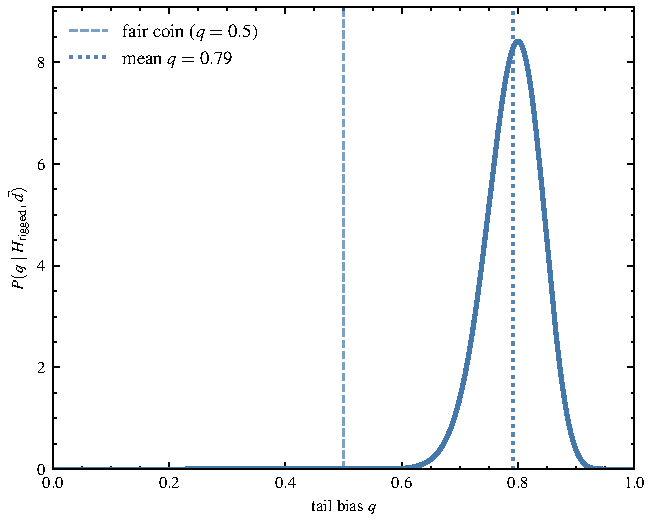
\includegraphics[width=\textwidth,height=0.9\textheight,keepaspectratio]{cointossposterior.pdf}
		\end{column}
		\hfill
		\begin{column}{0.7\textwidth}\large
			\vspace{-2em}
			\cc{What can we tell about the coin?}
			$$P(q|H_\text{rigged},\vec d) = \frac{P(\vec d|H_\text{rigged},q) \cdot P(q|H_\text{rigged})}{P(\vec d|H_\text{rigged})}$$
			%$$= \frac{\prod_{i=1}^{10} P(d_i|H_\text{rigged},q) \cdot P(q|H_\text{rigged})}{P(\vec d|H_\text{rigged})}$$
			%$$= \frac{\prod_{i=1}^{10} \binom{N}{T} \cdot q^T \cdot (1-q)^{N-T}}{P(\vec d|H_\text{rigged})}$$
			%The posterior distribution of $q$ is a Beta distribution with parameters $\alpha = 80 + 1$ and $\beta = 20 + 1$.
			%$$P(q|H_\text{rigged},\vec d) = \frac{\Gamma(\alpha+\beta)}{\Gamma(\alpha)\Gamma(\beta)} q^{\alpha-1} (1-q)^{\beta-1}$$
			%The mean of the posterior distribution is $\alpha/(\alpha+\beta) = 0.8$.
			%\cc{The coin is likely rigged, and the bias is likely around 0.8.}
		\end{column}
	\end{columns}
\end{frame}

\begin{frame}{Summary}
	\vspace{-2em}
	\begin{columns}[T]
		\begin{column}{0.4\textwidth}
			\centering
			\includegraphics[width=\textwidth,height=0.9\textheight,keepaspectratio]{cointoss.png}
		\end{column}
		\hfill
		\begin{column}{0.7\textwidth}\large
			\vspace{-2em}
			\cc{Summary}
			\ccc{Bayes factor is the ratio of the likelihood of the data under two competing hypotheses.}
			\ccc{Bayes factor alone is not enough to determine which hypothesis is more likely. We also need to consider the prior odds.}
			\ccc{The posterior odds is the product of the Bayes factor and the prior odds.}
			\ccc{The coin in Macau is probably not rigged, but a coin in a home casino with similar data is probably rigged.}
			\ccc{We can also estimate the bias of the coin using the posterior distribution of $q$.}
		\end{column}
	\end{columns}
\end{frame}

\begin{frame}{Open question: Detection of lensing}
	\cc{Suppose that a gravitational-wave signal is detected}
	\ccc{We analyse the signal under "microlensing" and "regular" hypotheses}
	\cc{Bayes factor is around 100}
	\cc{Is the signal microlensed?}
	\ccc{What are the factors that we need to consider to answer this question?}
\end{frame}

\end{document}

